% Every number below is a macro generated from saved analysis files by scripts/build_camera_ready_assets.py.
\subsection{Reproducibility and Executed Budgets}
All \R{hc-budget-exact} HalfCheetah and \R{ant-budget-exact} Ant branches ran exactly 20,000 steps and 5,000 updates. The \R{hc-repro-branches} HalfCheetah branches that share their seeds with the pilot reproduce its returns at 0, 2,000 and 4,000 steps exactly (largest absolute difference \R{hc-repro-maxdiff}), and recomputing the pilot's metric from them returns its published means. After a memory failure, \R{rerun-branches} completed reactive branches were rerun from scratch; their evaluation returns and \R{rerun-ckpt-identical} of \R{rerun-branches} final checkpoints are bit-identical to the first run.

\begin{figure}[tp]
\centering
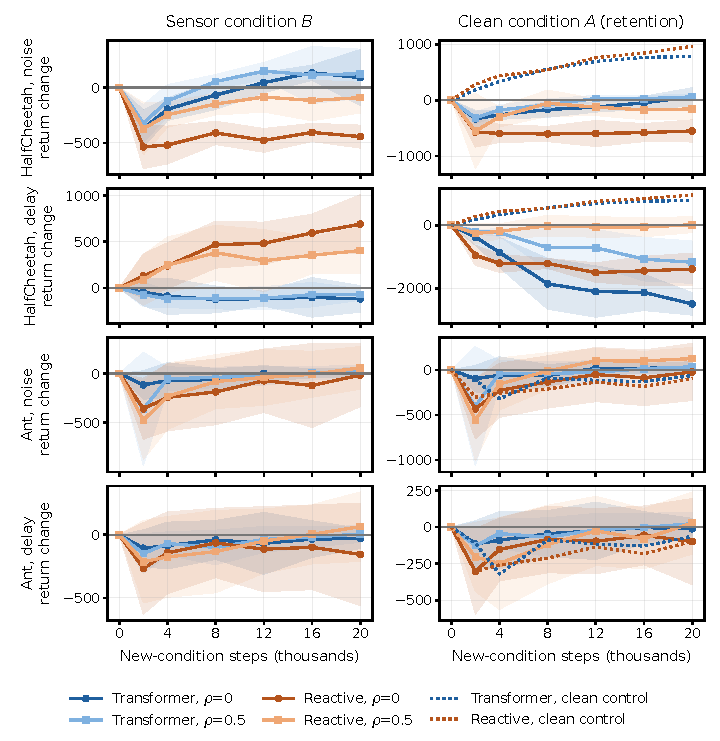
\includegraphics[width=\textwidth]{fig_curves.pdf}
\caption{Mean change in sensor-condition return (left) and clean-condition return (right) during continued training in HalfCheetah (top two rows) and Ant (bottom two rows), with 95\% $t$ intervals over eight source seeds. Dotted lines are the clean-continuation controls.}
\label{fig:curves}
\end{figure}

\begin{table}[t]
\caption{Outcomes at 20,000 steps: mean over eight source seeds with 95\% $t$ intervals. $B(0)$ is the zero-step sensor-condition return; $\Delta B$ and $\Delta A$ are the changes in sensor- and clean-condition return. For the clean control, $B=A$.}
\label{tab:outcomes}
\centering\scriptsize
\setlength{\tabcolsep}{3pt}
\begin{tabular*}{\textwidth}{@{\extracolsep{\fill}}llrrrr@{}}
\toprule
Controller & Fault & $\rho$ & $B(0)$ & $\Delta B$ [95\% CI] & $\Delta A$ [95\% CI] \\
\midrule
\multicolumn{6}{@{}l}{\emph{HalfCheetah-v5}} \\
Transformer & Noise & 0 & 2{,}402 & +89 [\ensuremath{-}163, 341] & +59 [\ensuremath{-}104, 222] \\
Transformer & Noise & 0.5 & 2{,}402 & +125 [\ensuremath{-}96, 346] & +59 [14, 104] \\
Transformer & Delay & 0 & 13 & \ensuremath{-}115 [\ensuremath{-}259, 28] & \ensuremath{-}2{,}496 [\ensuremath{-}2{,}852, \ensuremath{-}2{,}139] \\
Transformer & Delay & 0.5 & 13 & \ensuremath{-}69 [\ensuremath{-}130, \ensuremath{-}9] & \ensuremath{-}1{,}173 [\ensuremath{-}1{,}846, \ensuremath{-}500] \\
Transformer & Clean control & 0 & 2{,}695 & --- & +782 [606, 958] \\
Reactive & Noise & 0 & 2{,}900 & \ensuremath{-}443 [\ensuremath{-}546, \ensuremath{-}339] & \ensuremath{-}550 [\ensuremath{-}748, \ensuremath{-}352] \\
Reactive & Noise & 0.5 & 2{,}900 & \ensuremath{-}91 [\ensuremath{-}230, 47] & \ensuremath{-}157 [\ensuremath{-}339, 26] \\
Reactive & Delay & 0 & \ensuremath{-}179 & +689 [373, 1{,}006] & \ensuremath{-}1{,}390 [\ensuremath{-}1{,}896, \ensuremath{-}884] \\
Reactive & Delay & 0.5 & \ensuremath{-}179 & +406 [153, 658] & +16 [\ensuremath{-}233, 266] \\
Reactive & Clean control & 0 & 3{,}239 & --- & +963 [740, 1{,}187] \\
\addlinespace[2pt]
\multicolumn{6}{@{}l}{\emph{Ant-v5}} \\
Transformer & Noise & 0 & 921 & +7 [\ensuremath{-}46, 61] & +27 [\ensuremath{-}37, 90] \\
Transformer & Noise & 0.5 & 921 & +22 [\ensuremath{-}40, 85] & +34 [\ensuremath{-}38, 105] \\
Transformer & Delay & 0 & 918 & \ensuremath{-}30 [\ensuremath{-}110, 50] & \ensuremath{-}12 [\ensuremath{-}83, 59] \\
Transformer & Delay & 0.5 & 918 & +6 [\ensuremath{-}60, 72] & +22 [\ensuremath{-}58, 102] \\
Transformer & Clean control & 0 & 899 & --- & \ensuremath{-}64 [\ensuremath{-}187, 60] \\
Reactive & Noise & 0 & 651 & \ensuremath{-}16 [\ensuremath{-}338, 305] & \ensuremath{-}24 [\ensuremath{-}341, 293] \\
Reactive & Noise & 0.5 & 651 & +57 [\ensuremath{-}159, 274] & +125 [1, 250] \\
Reactive & Delay & 0 & 588 & \ensuremath{-}156 [\ensuremath{-}562, 251] & \ensuremath{-}100 [\ensuremath{-}393, 194] \\
Reactive & Delay & 0.5 & 588 & +64 [\ensuremath{-}211, 339] & +27 [\ensuremath{-}185, 239] \\
Reactive & Clean control & 0 & 674 & --- & \ensuremath{-}98 [\ensuremath{-}376, 180] \\
\bottomrule
\end{tabular*}
\end{table}


\subsection{HalfCheetah}
Table~\ref{tab:outcomes} lists the outcomes and Fig.~\ref{fig:curves} (top rows) shows their course. Before continued training, noise reduced the mean return of the transformer sources from \R{hc-transformer-A0} to \R{hc-transformer-noise-0-B0} and that of the reactive sources from \R{hc-reactive-A0} to \R{hc-reactive-noise-0-B0}, whereas delay reduced it to \R{hc-transformer-delay-0-B0} and \R{hc-reactive-delay-0-B0}. Continued clean training raised clean return by \R{hc-transformer-clean-0-dA} and \R{hc-reactive-clean-0-dA}, with every seed improving. The sources were therefore not converged, and the clean control, not $\Delta^A=0$, is the reference for fault-specific forgetting.

\paragraph{Adaptation.} Under delay, the reactive controller's delayed-sensing return rose by \R{hc-reactive-delay-0-dB} \R{hc-reactive-delay-0-dB-ci} with every seed improving, to \R{hc-reactive-delay-0-B1}, still far below its clean return. The transformer did not improve under delay (\R{hc-transformer-delay-0-dB} \R{hc-transformer-delay-0-dB-ci}). Under noise, both controllers first lost return. The transformer recovered to \R{hc-transformer-noise-0-dB} \R{hc-transformer-noise-0-dB-ci} by 20,000 steps, whereas the reactive controller stayed below its starting value (\R{hc-reactive-noise-0-dB} \R{hc-reactive-noise-0-dB-ci}, all seeds).

\paragraph{Retention.} Without retained replay, every fault branch ended below the clean control on clean data. The differences are \R{hc-FS-transformer-noise} under noise and \R{hc-FS-transformer-delay} under delay for the transformer, and \R{hc-FS-reactive-noise} and \R{hc-FS-reactive-delay} for the reactive controller. All eight seeds agree in each case (Holm-adjusted $p=\R{hc-FS-transformer-noise-holm}$, the floor of this family). Relative to the sources, clean return fell under delay (\R{hc-transformer-delay-0-dA} and \R{hc-reactive-delay-0-dA}) and, for the reactive controller, under noise (\R{hc-reactive-noise-0-dA}). The transformer's clean return under noise ended near its starting value (\R{hc-transformer-noise-0-dA} \R{hc-transformer-noise-0-dA-ci}).

\paragraph{Retained replay.} Retained replay reduced each clean-condition loss (Table~\ref{tab:tests}). The paired effect on $\Delta^A$ was $D=\R{hc-D-transformer-delay-dA}$ for the transformer under delay, and $D=\R{hc-D-reactive-delay-dA}$ and $D=\R{hc-D-reactive-noise-dA}$ for the reactive controller under delay and noise, with all eight seeds positive in each case. With $\rho=0.5$, the reactive controller's clean return under delay ended at its source value (\R{hc-reactive-delay-50-dA} \R{hc-reactive-delay-50-dA-ci}), and its noise-condition decline also shrank ($D=\R{hc-D-reactive-noise-dB}$, all seeds). The cost appeared under delay. Replay reduced the reactive controller's delayed-sensing gain ($D=\R{hc-D-reactive-delay-dB}$, \R{hc-D-reactive-delay-dB-ci}; \R{hc-D-reactive-delay-dB-neg} of 8 seeds negative), the trade-off seen in the pilot. For the transformer, replay left the delayed-sensing outcome unchanged ($D=\R{hc-D-transformer-delay-dB}$, \R{hc-D-transformer-delay-dB-ci}) and changed neither outcome under noise. Each consistent effect has exact $p=\R{hc-D-transformer-delay-dA-p}$ and Holm-adjusted $p=\R{hc-D-transformer-delay-dA-holm}$, the floor for eight tests with eight seeds.

\paragraph{Comparison with the pilot.} The three-seed pilot had shown a small transformer gain under delay after 4,000 steps (\R{hc-transformer-delay-0-dB-pilot4k}). With eight seeds and five evaluation episodes, the change at that budget is \R{hc-transformer-delay-0-dB-4k} (\R{hc-transformer-delay-0-dB-4k-neg} of 8 seeds negative), and it remains negative through 20,000 steps. The reactive controller's delay gain and both controllers' clean-condition losses under delay persist and grow with the longer budget.

\begin{table}[t]
\caption{Pre-specified paired replay effect $D=\text{metric}(\rho{=}0.5)-\text{metric}(\rho{=}0)$ at 20,000 steps (eight seeds). Holm-adjusted exact Wilcoxon $p$ within each task's eight tests; $+/-$ counts seeds with positive and negative $D$.}
\label{tab:tests}
\centering\scriptsize
\setlength{\tabcolsep}{3pt}
\begin{tabular*}{\textwidth}{@{\extracolsep{\fill}}llrrrrrr@{}}
\toprule
Controller & Fault & $D_{\Delta A}$ [95\% CI] & $p_\text{Holm}$ & $+/-$ & $D_{\Delta B}$ [95\% CI] & $p_\text{Holm}$ & $+/-$ \\
\midrule
\multicolumn{8}{@{}l}{\emph{HalfCheetah-v5}} \\
Transformer & Noise & 0 [\ensuremath{-}158, 159] & 1.00 & 5/3 & +36 [\ensuremath{-}63, 134] & 1.00 & 5/3 \\
Transformer & Delay & +1{,}323 [595, 2{,}050] & 0.0625 & 8/0 & +46 [\ensuremath{-}102, 195] & 1.00 & 5/3 \\
Reactive & Noise & +394 [188, 599] & 0.0625 & 8/0 & +351 [153, 549] & 0.0625 & 8/0 \\
Reactive & Delay & +1{,}406 [816, 1{,}997] & 0.0625 & 8/0 & \ensuremath{-}284 [\ensuremath{-}567, \ensuremath{-}1] & 0.31 & 2/6 \\
\addlinespace[2pt]
\multicolumn{8}{@{}l}{\emph{Ant-v5}} \\
Transformer & Noise & +7 [\ensuremath{-}21, 35] & 1.00 & 4/4 & +15 [\ensuremath{-}3, 32] & 0.55 & 6/2 \\
Transformer & Delay & +34 [\ensuremath{-}27, 96] & 1.00 & 4/4 & +36 [\ensuremath{-}31, 103] & 1.00 & 5/3 \\
Reactive & Noise & +149 [\ensuremath{-}116, 414] & 1.00 & 6/2 & +74 [\ensuremath{-}135, 282] & 1.00 & 5/3 \\
Reactive & Delay & +127 [\ensuremath{-}61, 315] & 1.00 & 5/3 & +220 [\ensuremath{-}34, 474] & 0.31 & 7/1 \\
\bottomrule
\end{tabular*}
\end{table}


\subsection{Ant}
\paragraph{Sources.} Under the same recipe, every Ant source learned to stand rather than walk. Across the 16 sources, the mean forward velocity in clean evaluation never exceeded \R{ant-xvel-absmax}\,m/s in magnitude, every clean evaluation episode lasted 1,000 steps, and the source returns (\R{ant-transformer-A0} for the transformer and \R{ant-reactive-A0} for the reactive controller) come mainly from Ant's healthy reward of one per step. Standing proved robust to the faults. Zero-step sensor-condition returns were \R{ant-transformer-noise-0-B0} under noise and \R{ant-transformer-delay-0-B0} under delay for the transformer, and \R{ant-reactive-noise-0-B0} and \R{ant-reactive-delay-0-B0} for the reactive controller, whose delayed-sensing episodes ended early in \R{ant-reactive-term0-delay}\% of evaluations. Ant therefore tests retention during continued training more than adaptation.

\paragraph{Continued training.} In every arm, mean return on both conditions fell during the first 2,000 steps (Fig.~\ref{fig:curves}, bottom rows), including the clean controls (\R{ant-transformer-clean-0-dA-2k} and \R{ant-reactive-clean-0-dA-2k}), and then recovered partly or fully. Because the clean controls dipped as well, this transient comes from restarting training rather than from the faults; in HalfCheetah, the clean controls improved at every budget. At 20,000 steps, every 95\% interval for the change in sensor-condition return included zero (Table~\ref{tab:outcomes}). Continued clean training did not improve the standing sources: clean return changed by \R{ant-transformer-clean-0-dA} \R{ant-transformer-clean-0-dA-ci} for the transformer and \R{ant-reactive-clean-0-dA} \R{ant-reactive-clean-0-dA-ci} for the reactive controller. The fault-specific contrasts, all negative in HalfCheetah, were therefore positive or near zero. The transformer's noise branches ended above the clean control on clean data by \R{ant-FS-transformer-noise} \R{ant-FS-transformer-noise-ci}, with all eight seeds agreeing (Holm-adjusted $p=\R{ant-FS-transformer-noise-holm}$, the floor); the other three intervals included zero.

\paragraph{Retained replay.} All eight paired replay effects had positive means, but every $t$ interval included zero (Table~\ref{tab:tests}). The most consistent was the effect on the reactive controller's delayed-sensing return ($D=\R{ant-D-reactive-delay-dB}$, \R{ant-D-reactive-delay-dB-ci}; \R{ant-D-reactive-delay-dB-pos} of 8 seeds positive; Holm-adjusted $p=\R{ant-D-reactive-delay-dB-holm}$). Without replay, that return changed by \R{ant-reactive-delay-0-dB} and \R{ant-reactive-delay-0-termfin-B}\% of delayed-sensing episodes ended early at 20,000 steps; with replay, \R{ant-reactive-delay-50-termfin-B}\% did. This effect has the opposite sign to HalfCheetah's, where replay reduced the delayed-sensing gain. With replay, the reactive controller's clean return under noise rose by \R{ant-reactive-noise-50-dA} \R{ant-reactive-noise-50-dA-ci}, with all eight seeds improving.

\begin{table}[t]
\caption{Critic diagnostic (mean over eight seeds) at the source checkpoint and after 20,000 steps with $\rho=0$ or $0.5$: root-mean-square held-out soft Bellman residual on clean ($A$) and corrupted ($B$) evaluation data, and the value-bias gap, the Monte-Carlo bias on $B$ data minus that on $A$ data of the same checkpoint (positive: values on corrupted data are overestimated relative to clean data; exploratory).}
\label{tab:bias}
\centering\scriptsize
\setlength{\tabcolsep}{2pt}
\begin{tabular*}{\textwidth}{@{\extracolsep{\fill}}llrrrrrrrrr@{}}
\toprule
 & & \multicolumn{3}{c}{Residual, clean data $A$} & \multicolumn{3}{c}{Residual, corrupted data $B$} & \multicolumn{3}{c}{Value-bias gap $B-A$} \\
\cmidrule(lr){3-5}\cmidrule(lr){6-8}\cmidrule(l){9-11}
Controller & Fault & Source & $\rho{=}0$ & $\rho{=}0.5$ & Source & $\rho{=}0$ & $\rho{=}0.5$ & Source & $\rho{=}0$ & $\rho{=}0.5$ \\
\midrule
\multicolumn{11}{@{}l}{\emph{HalfCheetah-v5}} \\
Transformer & Noise & 0.58 & 0.58 & 0.61 & 4.25 & 1.13 & 1.49 & +27 & +18 & +13 \\
Transformer & Delay & 0.58 & 1.61 & 2.87 & 4.36 & 0.96 & 1.38 & +171 & +27 & +89 \\
Reactive & Noise & 1.55 & 1.04 & 1.72 & 6.89 & 1.81 & 3.40 & +28 & +19 & +23 \\
Reactive & Delay & 1.55 & 3.07 & 2.73 & 5.84 & 1.91 & 3.61 & +268 & +114 & +204 \\
\addlinespace[2pt]
\multicolumn{11}{@{}l}{\emph{Ant-v5}} \\
Transformer & Noise & 2.16 & 0.23 & 0.30 & 3.48 & 0.44 & 0.58 & \ensuremath{-}2 & 0 & \ensuremath{-}2 \\
Transformer & Delay & 2.16 & 1.35 & 0.34 & 1.16 & 0.27 & 0.28 & \ensuremath{-}1 & 0 & \ensuremath{-}1 \\
Reactive & Noise & 1.06 & 0.28 & 0.22 & 5.56 & 1.00 & 0.97 & +2 & +2 & +8 \\
Reactive & Delay & 1.06 & 0.72 & 3.05 & 2.00 & 3.03 & 1.23 & 0 & +15 & +3 \\
\bottomrule
\end{tabular*}
\end{table}


\subsection{Critic Diagnostic}
Table~\ref{tab:bias} reports the diagnostic, which is not part of the pre-specified analysis; the value-bias gap is exploratory. At the HalfCheetah sources, the held-out soft Bellman residual on corrupted data was several times that on clean data, and continued training on corrupted data reduced it in every arm. Retained replay raised the reactive controller's residual on corrupted data under both faults (by \R{hc-belD-reactive-noise-B} under noise and \R{hc-belD-reactive-delay-B} under delay, all eight seeds each; Holm-adjusted $p=\R{hc-belD-reactive-delay-B-holm}$, the floor) and its clean-data residual under noise (\R{hc-belD-reactive-noise-A}, all seeds). For the transformer, only the increase on noisy data had an interval excluding zero (\R{hc-belD-transformer-noise-B} \R{hc-belD-transformer-noise-B-ci}). In Ant, replay raised neither residual consistently; it lowered the transformer's clean-data residual under delay (\R{ant-belD-transformer-delay-A}, all eight seeds).

The value-bias gap separates the faults. The HalfCheetah source critics overvalued delayed-sensing histories relative to clean ones by \R{hc-gap-transformer-delay-src} (transformer) and \R{hc-gap-reactive-delay-src} (reactive), with all eight seeds positive in both, against \R{hc-gap-transformer-noise-src} and \R{hc-gap-reactive-noise-src} under noise. Training on delayed data alone shrank this gap to \R{hc-gap-transformer-delay-0} and \R{hc-gap-reactive-delay-0}. With retained replay it stayed larger, at \R{hc-gap-transformer-delay-50} and \R{hc-gap-reactive-delay-50}: paired effects of \R{hc-gapD-transformer-delay} \R{hc-gapD-transformer-delay-ci} and \R{hc-gapD-reactive-delay} \R{hc-gapD-reactive-delay-ci} (\R{hc-gapD-transformer-delay-pos} and \R{hc-gapD-reactive-delay-pos} of 8 seeds positive). Under noise, replay changed the gap by only \R{hc-gapD-transformer-noise} (transformer) and \R{hc-gapD-reactive-noise} (reactive). In Ant, every mean gap stayed within \R{ant-gap-absmax} return units of zero.

\begin{table}[t]
\caption{Per-action inference latency (ms) of the HalfCheetah source controllers (seed 42), batch size one, real model inputs, simulation excluded; 10{,}000 timed steps after warm-up on an AMD Ryzen 9 8940HX CPU and a GeForce RTX 5070 Laptop GPU. The transformer recomputes its full 32-token context at every step.}
\label{tab:latency}
\centering\small
\begin{tabular}{@{}llrrrr@{}}
\toprule
Controller & Device & Mean & p95 & p99 & Max \\
\midrule
Transformer & CPU, 1 thread & 0.58 & 0.62 & 0.66 & 1.56 \\
Transformer & CPU, 4 threads & 0.58 & 0.62 & 0.73 & 1.46 \\
Transformer & GPU & 1.64 & 1.72 & 1.79 & 3.03 \\
Reactive & CPU, 1 thread & 0.09 & 0.11 & 0.13 & 0.53 \\
Reactive & CPU, 4 threads & 0.09 & 0.11 & 0.13 & 0.48 \\
Reactive & GPU & 0.48 & 0.53 & 0.56 & 0.94 \\
\bottomrule
\end{tabular}
\end{table}


\subsection{Inference Latency}
Table~\ref{tab:latency} lists the per-action latency. On one CPU thread the transformer took \R{lat-transformer-cpu1-mean}\,ms on average and \R{lat-transformer-cpu1-p99}\,ms at the 99th percentile, and no timed CPU call exceeded \R{lat-transformer-cpu1-max}\,ms. Every CPU call therefore fit the 2\,ms period of 500\,Hz control, and the 10\,ms period of 100\,Hz control by a wide margin; the reactive controller took \R{lat-reactive-cpu1-mean}\,ms. Four threads brought no gain. At batch size one the GPU was slower than the CPU (\R{lat-transformer-gpu-mean}\,ms mean and \R{lat-transformer-gpu-max}\,ms maximum for the transformer), consistent with per-call launch and transfer overhead dominating such small networks. The figures cover the network call on a laptop workstation, not a complete control loop or an embedded processor.
